%%%%%%%%%%%%%%%%%%%%%%%%%%%%%%%%%%%%%%%%%%%%%%%%%%%%%%%%%%%%%
%
%  Figure 8.2
%
%%%%%%%%%%%%%%%%%%%%%%%%%%%%%%%%%%%%%%%%%%%%%%%%%%%%%%%%%%%%%


\begin{document}

\title{Triangle shape space}

\author{ }

\date{}

\maketitle


\vskip 0.5 cm


\begin{figure}[htbp]
\centering
\resizebox{7.5cm}{4.8cm}{%
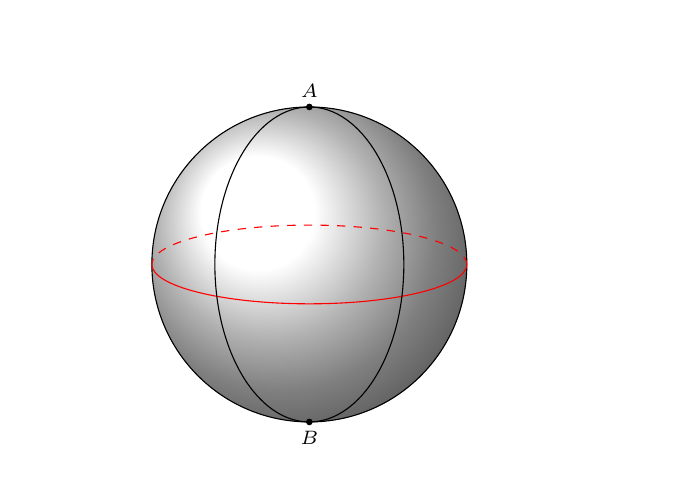
\begin{tikzpicture}
[
  point/.style = {draw, circle, fill=black, inner sep=0.7pt},
]
\def\rad{2cm}

\coordinate (O) at (0,0); %center of sphere
\coordinate (N) at (0,\rad); %x
\coordinate (R) at (\rad-32,0.4); %X'
\coordinate (TR) at (0.923*\rad,1.4*\rad-20);%Q
\coordinate (RR) at (-0.923*\rad+15,0.282*\rad);
\coordinate (O) at (0,0); %center of sphere
\coordinate (B) at (0,\rad); %x
\coordinate (C) at ({0.6*\rad*cos(-20)+1.5},{0.6*\rad*sin(-20)}); %X'
\coordinate (D) at (0,-\rad);%Q
\coordinate (E) at ({-0.6*\rad*cos(30)},{0.6*\rad*sin(30)}); %M

%ball
\filldraw[ball color=white] (O) circle [radius=\rad];
\draw[dashed, red] 
  (\rad,0) arc [start angle=0,end angle=180,x radius=\rad,y radius=5mm];
  %

  %black line round middle
\draw[red]
  (\rad,0) arc [start angle=0,end angle=-180,x radius=\rad,y radius=5mm];
    

 \draw[black]
  (B) arc [start angle=90,end angle=-90,x radius={\rad*0.6},y radius=20mm];
  
 \draw[black]
  (B) arc [start angle=90,end angle=-90,x radius=-{\rad*0.6},y radius=20mm];     
         
  %
  %\node[black] at (1,1.3) {$\gamma$};  
\begin{scope}[xslant=0.5,yshift=\rad,xshift=-2]
\filldraw[fill=gray!50,opacity=0]
  (-4,1) -- (3,1) -- (3,-1) -- (-4,-1) -- cycle; 
\end{scope}
%\node[point] at (A) {};
\node[point] at (B) {};
\node[point] at (D) {};
\draw (B)node[above]{$\scriptstyle{A}$};
\draw (D)node[below]{$\scriptstyle{B}$};
\end{tikzpicture}
}
\caption{\footnotesize{\textit{ }}}\label{fig:partransport}
\end{figure}

\end{document}